\chapter{Intelligent Student AI Hub: An Integrated Learning Platform} 
\label{chap:Student_AI_Hub}
\textbf{Author:} Luna Schaetzle

This chapter presents an in-depth overview of the Intelligent Student AI Hub, 
a comprehensive web platform designed to empower students in exploring Artificial Intelligence (AI) concepts. 
The platform integrates state-of-the-art technologies and innovative features to facilitate both learning and practical experimentation in AI. 
The following sections detail the system architecture, core functionalities, and future directions for this educational tool.

\section{Introduction}

The Intelligent Student AI Hub provides a robust environment for students to learn about AI and its real-world applications. 
It offers a diverse range of educational resources—including articles, tutorials, and interactive tools—to foster a deep understanding of AI concepts. 
By combining engaging content with advanced technological integration, the platform aims to make AI accessible, dynamic, and relevant to learners at all levels.

\section{System Architecture and Technologies}

This section outlines the principal technologies that form the backbone of the Intelligent Student AI Hub. By employing a combination of modern web frameworks and cloud-based services, the platform achieves a secure, scalable, and high-performance architecture.

\subsection{Vue.js}


The frontend of the platform is primarily developed using Vue.js—a progressive JavaScript framework renowned for its component-based structure and reactive data binding. Utilizing standard web technologies such as HTML, CSS, and JavaScript, Vue.js enables the creation of dynamic, single-page applications that are both modular and easy to maintain. For additional details on the implementation of HTML, JavaScript and CSS, please refer to Chapter \ref{chap:used_programming_languages}, subsection "Vue.js."

\subsection{Flask API}

The backend infrastructure is powered by a custom-developed Flask API. This API manages client requests and facilitates communication with a suite of self-hosted AI models and tools. Through efficient data handling and secure request management, the Flask API forms a critical link between the frontend interface and the underlying AI services. More comprehensive insights into the backend architecture are available in Chapter \ref{cha:hosted_flask_service}.

\subsection{ChatGPT API}

To augment the platform's interactive capabilities, the Intelligent Student AI Hub integrates the ChatGPT API via the OpenAI library. This integration supports a sophisticated chatbot feature that enables students to ask questions and receive detailed, context-aware responses on a variety of AI-related topics. Further information on this integration can be found in Chapter \ref{cha:Introduction_to_the_used_Large_Language_Models}, subsection "Integration of OpenAI's API."

\subsection{Firebase for Authentication and Data Storage}

For secure user management and efficient data handling, the platform employs Firebase services. 
Firebase Authentication provides a flexible and robust solution for verifying user identities through multiple sign-in methods—including email/password, 
third-party providers, and anonymous authentication. Additionally, Firebase’s real-time database and Cloud Firestore facilitate scalable and responsive data storage, 
synchronization, and retrieval. The seamless integration of Firebase with Vue.js components ensures that user data and authentication states are managed in real time, 
enhancing both security and user experience.

\cite{Firebase-features}


\section{Core Functionalities}

To get a comprehensive understanding of the Intelligent Student AI Hub, this section delves into its core functionalities and interactive features of the end product.
Some of the key features of the platform include:
\begin{itemize}
    \item \textbf{Interactive Chatbot for AI Questions:} The platform hosts an AI-powered chatbot that can answer a wide range of AI-related queries, providing students with instant access to information and explanations.
    \item \textbf{OpenAI Integration:} By integrating OpenAI’s cutting-edge models, such as ChatGPT and DALL-E, the platform offers advanced AI capabilities for generating text and images, enhancing the learning experience.
    \item \textbf{Programming Bot for Different Languages:} A specialized bot is available to assist students in learning and practicing various programming languages, offering code snippets, explanations, and interactive coding exercises.
    \item \textbf{Image Recognition Tool:} The platform includes an image recognition tool that leverages AI algorithms to identify objects, scenes, and patterns within uploaded images, enabling students to explore computer vision concepts.
    \item \textbf{Image-to-Text Tool:} Students can utilize an image-to-text tool that converts text embedded within images into editable and searchable content, facilitating the extraction of information from visual data.
    \item \textbf{Saved Chats:} The platform allows users to save and revisit previous chat interactions with the AI chatbot, enabling seamless continuity in learning and knowledge retention.
    \item \textbf{User Profiles and Authentication:} Each user can create a personalized profile, manage their learning progress, and access customized content based on their preferences and history.
\end{itemize}

\section{Authentication and User Profiles}

For the Intelligent Student AI Hub, Firebase is a cornerstone technology for managing user authentication and profile creation, ensuring both secure access and a personalized user experience.

\subsection{Why Firebase?}

Although numerous alternatives exist for user authentication and data management, Firebase distinguishes itself through its comprehensive feature set, 
seamless integration, and robust security measures. Additionally, the abundance of tutorials and detailed documentation facilitates a swift onboarding process for the development team.

\subsection{Firebase Authentication Factors}

Implementing robust authentication and user profile management involves several critical aspects:

\begin{itemize}
    \item \textbf{Firebase Authentication:} The platform leverages Firebase Authentication to facilitate secure user sign-in and verification. By supporting multiple authentication methods—including email/password, social logins (e.g., Google, Facebook), and anonymous authentication—Firebase offers a versatile solution that adapts to diverse user needs while ensuring a seamless and reliable experience.
    
    \item \textbf{Real-time Data Synchronization:} Utilizing Firebase’s Realtime Database and Cloud Firestore, the platform ensures that user data is consistently synchronized across all devices. This real-time updating mechanism provides immediate access to personalized content, settings, and user profiles, thus significantly enhancing user engagement.
    
    \item \textbf{Secure Data Handling:} Firebase incorporates robust security measures, including data encryption, secure authentication tokens, and finely tuned access control rules. These features work together to protect user data from unauthorized access, maintaining both data integrity and user privacy in accordance with best practices and regulatory requirements.
    
    \item \textbf{Integration with Vue.js Components:} The tight integration between Firebase and Vue.js enables dynamic data binding and responsive user interfaces. Leveraging Vue.js reactivity in combination with Firebase’s real-time updates results in a fluid user experience, where UI elements automatically refresh to reflect the most current state of user data.
    
    \item \textbf{Future Enhancements:} As the platform evolves, additional features such as recommendation engines, learning analytics, and collaborative learning tools could be integrated. These enhancements would further tailor content to individual user needs and foster a more engaging and personalized educational environment.
\end{itemize}

\subsection{Firebase Integration with Vue.js}

The integration of Firebase services within Vue.js is essential to achieving a seamless, interactive user experience on the Intelligent Student AI Hub. The process involves several key steps:

\begin{itemize}
    \item \textbf{Installing the Firebase SDK:} The Firebase JavaScript SDK is added to the Vue.js project via package managers like npm or yarn, providing access to Firebase’s suite of services directly within the application.
    
    \item \textbf{Initializing Firebase:} The SDK is initialized using project-specific configuration settings, including API keys, authentication methods, and database URLs. This step establishes a secure connection between the Vue.js application and Firebase services.
    
    \item \textbf{Implementing Authentication:} Vue.js components integrate Firebase Authentication methods to handle various sign-in options. These components are responsible for managing user sessions and ensuring secure access to personalized content and features.
    
    \item \textbf{Managing User Profiles:} User-specific data—such as preferences, settings, and learning progress—is stored in Firebase databases. Vue.js components interact with these services to create, update, and retrieve profiles, with real-time synchronization ensuring that updates are reflected immediately across all user devices.
    
    \item \textbf{Handling Real-time Updates:} Vue.js reactivity is combined with Firebase’s real-time data listeners. This ensures that any changes in user data trigger immediate UI updates, thereby providing a consistently accurate and current view of the user’s profile and settings.
    
    \item \textbf{Implementing Security Rules:} Firebase security rules are configured to enforce strict access control policies. By restricting read and write permissions to authenticated users only, these rules help maintain data integrity and protect user privacy.
\end{itemize}

For the integration process, the VueJS Firebase library is utilized, streamlining the connection between Vue.js projects and Firebase. This library simplifies access to numerous Firebase features—including Authentication, Realtime Database, Firestore, Storage, and restricted pages for non-authenticated users—making it easier to implement a secure and efficient system.

\subsection{Implementation of Firebase Authentication}

A robust implementation of Firebase Authentication within Vue.js involves both proper configuration and thoughtful component design. The following code snippets illustrate key aspects of this integration.

\vspace{1em}
\textbf{Firebase Initialization and Authentication Setup:}

\begin{lstlisting}[language=JavaScript, caption={Initializing Firebase and setting up authentication}]
import firebase from 'firebase/app';
import 'firebase/auth';

// Firebase configuration object containing keys and identifiers
const firebaseConfig = {
  apiKey: "YOUR_API_KEY",
  authDomain: "YOUR_PROJECT_ID.firebaseapp.com",
  databaseURL: "https://YOUR_PROJECT_ID.firebaseio.com",
  projectId: "YOUR_PROJECT_ID",
  storageBucket: "YOUR_PROJECT_ID.appspot.com",
  messagingSenderId: "YOUR_SENDER_ID",
  appId: "YOUR_APP_ID"
};

// Initialize Firebase with the configuration
firebase.initializeApp(firebaseConfig);

// Export the authentication module for use in Vue components
export const auth = firebase.auth();

// Monitor authentication state changes
auth.onAuthStateChanged(user => {
  if (user) {
    // User is signed in; update application state accordingly
    console.log('User signed in:', user);
  } else {
    // User is signed out; update the UI to reflect sign-out state
    console.log('No user is signed in.');
  }
});
\end{lstlisting}

\vspace{1em}
\textbf{Explanation:}
\begin{itemize}
    \item \textbf{Firebase Import and Configuration:} The Firebase modules are imported, and the application is initialized using a configuration object that contains the necessary API keys and identifiers. This setup establishes the connection to Firebase services.
    \item \textbf{Authentication Monitoring:} The \texttt{onAuthStateChanged} listener is used to monitor changes in the user’s authentication state. This enables the application to dynamically update its interface in response to sign-in or sign-out events.
\end{itemize}

\vspace{1em}
\textbf{Vue.js Component Example with Authentication:}

\begin{lstlisting}[language=HTML, caption={Vue.js component for user sign-in}]
<template>
    <div>
        <!-- Display a welcome message if the user is signed in -->
        <h2 v-if="user">Welcome, {{ user.email }}</h2>
        <!-- Otherwise, show the sign-in form -->
        <div v-else>
            <input v-model="email" placeholder="Email" />
            <input v-model="password" type="password" placeholder="Password" />
            <button @click="signIn">Sign In</button>
            <button @click="signInWithGoogle">Sign In with Google</button>
            <p v-if="errorMessage" class="error">{{ errorMessage }}</p>
        </div>
    </div>
</template>

<script>
import { auth } from '@/firebase'; // Adjust the path according to your project structure
import firebase from 'firebase/app';
import 'firebase/auth';

export default {
    data() {
        return {
            email: '',
            password: '',
            user: null,
            errorMessage: ''
        };
    },
    created() {
        // Listen for authentication state changes and update the component state
        auth.onAuthStateChanged(user => {
            this.user = user;
        });
    },
    methods: {
        signIn() {
            // Attempt to sign in using the provided email and password
            auth.signInWithEmailAndPassword(this.email, this.password)
                .then(credential => {
                    this.user = credential.user;
                    this.errorMessage = '';
                })
                .catch(error => {
                    // Handle authentication errors by updating the errorMessage state
                    this.errorMessage = error.message;
                    console.error("Authentication error:", error);
                });
        },
        signInWithGoogle() {
            const provider = new firebase.auth.GoogleAuthProvider();
            auth.signInWithPopup(provider)
                .then(result => {
                    this.user = result.user;
                    this.errorMessage = '';
                })
                .catch(error => {
                    this.errorMessage = error.message;
                    console.error("Google sign-in error:", error);
                });
        }
    },
};
</script>

<style scoped>
.error {
    color: red;
    font-size: 0.9em;
}
</style>
\end{lstlisting}

\vspace{1em}
\textbf{Explanation:}
\begin{itemize}
    \item \textbf{Conditional Rendering:} The template uses Vue.js directives (\texttt{v-if} and \texttt{v-else}) to conditionally display content based on whether a user is authenticated. A personalized welcome message is shown when the user is signed in, while a sign-in form is presented otherwise.
    \item \textbf{Data Binding and State Management:} The component’s data properties (\texttt{email}, \texttt{password}, \texttt{user}, and \texttt{error messages}) are used to manage form inputs, the authenticated user state, and error messages.
    \item \textbf{Sign-In Method:} The \texttt{Sign-in} method invokes Firebase Authentication’s \texttt{signInWithEmailAndPassword} function. Proper error handling is implemented to provide feedback to the user in case of sign-in failures.
    \item \textbf{Real-time Authentication Updates:} The \texttt{onAuthStateChanged} listener, set up in the \texttt{created} hook, ensures that the component’s state is kept in sync with the authentication status, thereby reflecting any changes immediately in the UI.
    \item \textbf{Google Sign-In:} The \texttt{signInWithGoogle} method demonstrates how to enable Google sign-in using Firebase’s GoogleAuthProvider. This method follows a similar pattern to the email/password sign-in process.
    \item \textbf{Styling and Error Handling:} The component includes scoped styles for error messages and provides visual feedback to users when authentication errors occur.
\end{itemize}

\textbf{Best Practices and Future Considerations:}
\begin{itemize}
    \item \textbf{Error Handling and User Feedback:} Robust error handling is essential for providing clear user feedback and maintaining a secure application environment.
    \item \textbf{Scalability and Maintainability:} Modularizing the Firebase configuration and authentication logic allows for easier maintenance and future feature integrations, such as multi-factor authentication.
    \item \textbf{Security Enhancements:} Implementing advanced security measures, such as multi-factor authentication and periodic token refresh, can further enhance the platform’s security posture.
\end{itemize}

Through these implementations, the Intelligent Student AI Hub not only provides secure authentication and personalized user experiences but also lays the groundwork for future enhancements in user engagement and data security.

\subsection{User Overview and Personalization}

To enhance user engagement, the Intelligent Student AI Hub provides a personalized overview of each user's profile. This dedicated account management page consolidates essential information—including profile details, learning progress, and tailored recommendations—into a central hub that facilitates the management of user settings, preferences, and overall platform interactions.

\begin{figure}[H]
    \centering
    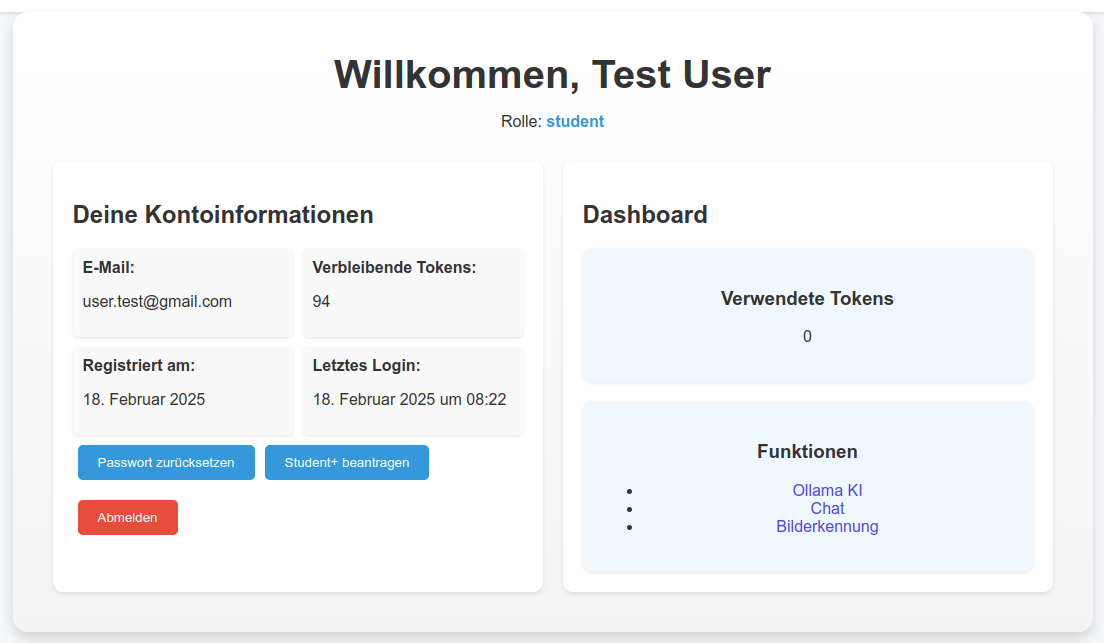
\includegraphics[width=0.8\textwidth]{figures/Account-Managment.png}
    \caption{User Account Management and Overview}
    \label{fig:user_account_management}
\end{figure}

\subsection{Outlook for Account Management}

Looking forward, there is considerable potential to expand the account management functionality with advanced features, such as:

\begin{itemize}
    \item \textbf{Enhanced Personalization:} Integration of sophisticated personalization tools, including dynamic content recommendations, curated learning paths, and detailed progress tracking, to provide a more tailored and effective learning experience.
    \item \textbf{Premium Account Options:} Introduction of premium account tiers that unlock advanced features and increase the allocation of request tokens for the ChatGPT API.
    \item \textbf{Social Integration:} Implementation of social login options, content sharing functionalities, and collaborative learning tools to foster a more interactive and community-driven environment.
    \item \textbf{Teacher Functionality:} Development of specialized tools for educators, enabling them to better manage classroom interactions and support student learning.
    \item \textbf{Administrator Dashboard:} Creation of a comprehensive administrative interface for efficient management of user accounts, content moderation, and platform analytics, thereby streamlining oversight and enhancing operational efficiency.
\end{itemize}

\subsection{TSN Integration}

Every student at HTL is provided with a TSN email account, which serves as the primary communication channel within the institution. During the development of the Student AI Hub, integrating the TSN email account was considered as a potential feature. However, after careful evaluation, we decided against this integration for several critical reasons:

\begin{itemize}
    \item \textbf{Security Concerns:} Incorporating the TSN email account would necessitate accessing sensitive user data. Without robust safeguards, this could significantly increase the risk of security breaches and data leakage.
    \item \textbf{Technical Complexity:} The integration would require the implementation of more sophisticated authentication mechanisms than those offered by Firebase. This added complexity could result in compatibility issues and pose significant challenges in terms of ongoing maintenance and support.
    \item \textbf{Impact on User Experience:} Requiring users to navigate additional authentication steps to access the platform could negatively affect the overall user experience. A more complicated login process may lead to reduced adoption rates and lower user satisfaction.
    \item \textbf{Regulatory and Compliance Challenges:} Ensuring compliance with data protection regulations and institutional policies would be more demanding with the TSN email integration. This approach would require addressing additional legal and technical considerations to maintain adherence to relevant standards.
\end{itemize}

\section{Interactive Chatbot for Day-to-Day AI Questions}

The objective of this feature is to provide students with immediate, context-aware responses to a broad spectrum of AI-related inquiries. To achieve this, the Intelligent Student AI Hub integrates multiple advanced Ollama AI models (e.g., LLaMA 3.2 and Mistral), enabling users to select the model that best fits the complexity and responsiveness required by their query. This modular approach ensures that students receive the most effective and contextually relevant answers, thereby enhancing their learning experience.

A self-hosted Flask API serves as the intermediary between the user interface and the Ollama API. This architecture allows the system to capture user input, forward the request to the selected AI model via the Flask API, and then relay the model's response back to the user in real time. The following abbreviated code listing illustrates the core implementation within a Vue.js component, demonstrating how the integration is achieved:

\begin{lstlisting}[language=html, caption={Abbreviated Vue.js Integration Example}, frame=single]
<template>
  <div>
    <!-- AI Model Selection -->
    <select v-model="selectedModel">
      <option value="llama3.2:1b">LLaMA 3.2 - 1B (Fast)</option>
      <option value="llama3.2">LLaMA 3.2 - 2B (Latest)</option>
      <!-- more Models -->
    </select>
    <!-- Chat Display -->
    <div v-for="msg in currentChat.messages" :key="msg.id">
      <p v-if="msg.type==='user'">{{ msg.text }}</p>
      <p v-else>{{ msg.text }}</p>
    </div>
    <!-- User Input and Submission -->
    <input v-model="userInput" @keydown.enter="sendMessage" placeholder="Ask the AI question..." />
    <button @click="sendMessage">Send</button>
  </div>
</template>

<script>
import axios from 'axios';
export default {
  data() {
    return {
      userInput: '',
      selectedModel: 'llama3.2:1b',
      currentChat: { messages: [] },
    };
  },
  methods: {
    async sendMessage() {
      if (!this.userInput.trim()) return;
      // Append user message to chat
      this.currentChat.messages.push({ id: Date.now(), type: 'user', text: this.userInput });
      // Send the query to the Flask API
      const response = await axios.post('http://server-address/ask_ollama', {
        prompt: this.userInput,
        model: this.selectedModel,
      });
      // Append AI response to chat
      this.currentChat.messages.push({ id: Date.now(), type: 'ollama', text: response.data.choices[0].text });
      this.userInput = '';
    },
  },
};
</script>
\end{lstlisting}

This example demonstrates the fundamental components of the integration:
\begin{itemize}
  \item \textbf{Model Selection:} A dropdown menu allows users to choose from various AI models, balancing speed and sophistication.
  \item \textbf{Real-Time Communication:} User inputs are captured and transmitted asynchronously to the Flask API, which then retrieves responses from the selected Ollama AI model.
  \item \textbf{Dynamic Chat Interface:} The chat interface updates dynamically with both user queries and AI responses, ensuring an engaging, real-time interaction.
\end{itemize}

By decoupling the frontend from the backend AI processing via a RESTful API, this design not only simplifies maintenance but also facilitates future scalability. New models or enhanced features can be integrated with minimal changes to the existing codebase, ensuring the platform remains adaptable to evolving educational needs.


\section{OpenAI Integration}

Given that locally hosted Ollama AI models may not achieve the same performance level as commercially available state-of-the-art solutions, 
the Intelligent Student AI Hub integrates advanced OpenAI models—such as ChatGPT and DALL-E—to deliver superior capabilities in text generation and image synthesis. 
This integration not only augments the quality of responses but also significantly enhances platform scalability. With the OpenAI API, 
scalability is effectively decoupled from hardware limitations, unlike the self-hosted Ollama API, which is inherently constrained by the available computational 
resources.

\subsection{ChatGPT API and Its Limitations}

A primary limitation of the ChatGPT API is the cost associated with each API request. 
Every query incurs a fee that can rapidly accumulate with high usage volumes. 

\begin{figure}[H]
    \centering
    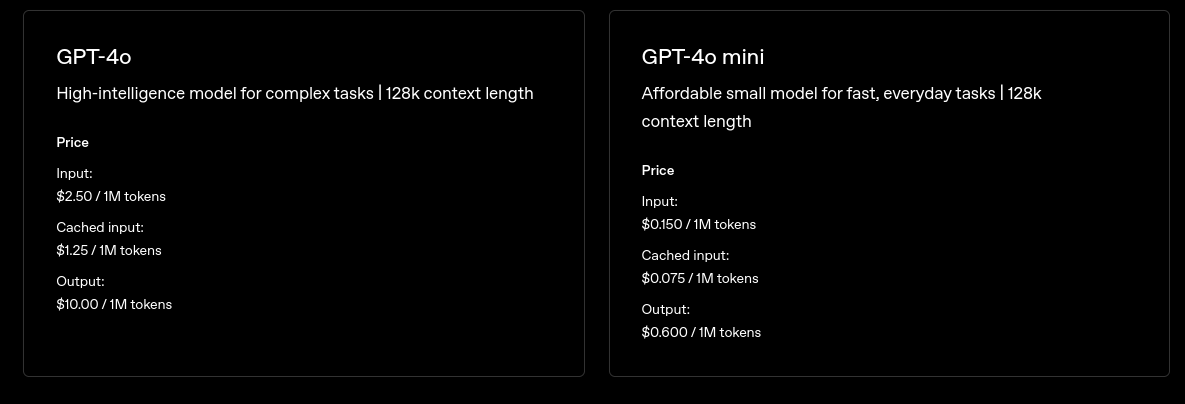
\includegraphics[width=0.8\textwidth]{figures/ChatGPT-API_Pricing.png}
    \caption{ChatGP API Pricing}
    \label{fig:chatgpt_api_integration}
\end{figure}

\cite{ChatGPT-API-Pricing}

For instance, utilizing ChatGPT-4o Mini costs \$0.30 per million input tokens, 
whereas the full ChatGPT-4o model incurs a cost of \$3.75 per million input tokens equating to a 12.5-fold increase in expense 
(see Figure~\ref{fig:chatgpt_api_integration}).
\footnote{Pricing data is current as of 17.02.2025 and may be subject to change.} 

Consequently, the development team has opted to restrict the use of the ChatGPT API. 
This measured approach enables students to benefit from ChatGPT’s advanced functionalities while effectively managing costs. 
Moreover, it is more economical for the institution to subsidize access to the API than to provide every student with an individual premium account.

\subsection{User Access to Paid Services}

Standard users are allocated a finite number of ChatGPT API requests per month, with these request tokens being replenished on a monthly basis. The number of tokens consumed per query is contingent upon the chosen model.
\footnote{Token allocations and model thresholds are periodically adjusted in response to current pricing structures and monthly usage limits.} 
Should a user exhaust their monthly token quota, they may alternatively direct their queries to the Ollama API. In addition to standard user access, premium, teacher, and administrator accounts are available, each benefiting from a higher monthly token allocation. Initially, all users are granted standard access; any desired upgrade to premium, teacher, or administrator status requires a formal request to the platform administration.

\subsection{Integration of OpenAI's API}

For a comprehensive guide on integrating OpenAI's API into a Vue.js project, please refer to Chapter \ref{cha:Introduction_to_the_used_Large_Language_Models}, Section \ref{sec:openai-api-implementation}.


\section{Programming Bot for Different Programming Languages}

The Intelligent Student AI Hub incorporates a dedicated programming bot designed to facilitate the learning and practice of various programming languages. Building upon the foundational architecture of the general chatbot, this bot leverages code-centric large language models (LLMs) that have been specifically trained on source code. As with the standard chatbot, users can select from different models that are optimized for programming-related tasks.

\textbf{Programming Bot Features}

Several enhancements have been integrated into the programming bot to improve its functionality and user experience:

\begin{itemize}
  \item \textbf{Programming Language Selection:} A dropdown menu enables users to specify the programming language for which they require assistance. The selected language is incorporated into the user’s query—modifying the prompt sent to the LLM—to ensure that responses are tailored appropriately. This modification is handled on the backend via a dedicated Flask API endpoint.
  
  \item \textbf{Prompt Refinement:} An integrated "refine" option allows users to modify their initial query. By clicking the refine button, users can adjust their question, prompting the LLM to generate a more precise response.
  
  \item \textbf{Code Rendering and Clipboard Functionality:} The frontend renders responses in Markdown, which facilitates automatic syntax highlighting of code blocks. Additionally, a "copy to clipboard" feature is provided, enabling users to easily extract and reuse the code samples.
\end{itemize}

Further details regarding the backend implementation are provided in Chapter \ref{cha:hosted_flask_service}.

\subsubsection{Markdown for Code Formatting}

Markdown is a lightweight markup language that supports plain-text formatting and can be easily converted into various output formats. Given that most LLM responses are delivered in Markdown, this feature simplifies the rendering of code with syntax highlighting. This approach is particularly useful for displaying well-formatted code snippets alongside explanatory text \cite{What-Is-Markdown}.

\paragraph{Illustrative Implementation Example:}

The following abbreviated Vue.js component demonstrates the key aspects of the programming bot integration. This example illustrates how the user can select a programming language, refine their input, and receive formatted code output:

\begin{lstlisting}[language=html, caption={Abbreviated Vue.js Component for the Programming Bot}, frame=single]
<template>
  <div class="programming-bot">
    <!-- Selection Area for Model and Programming Language -->
    <div class="selection-area">
      <select v-model="selectedModel">
        <option value="modelA">Model A</option>
        <option value="modelB">Model B</option>
      </select>
      <select v-model="selectedLanguage">
        <option value="python">Python</option>
        <option value="java">Java</option>
      </select>
    </div>
    <!-- Chat Interface -->
    <div class="chat-box">
      <div v-for="msg in messages" :class="msg.type">{{ msg.text }}</div>
    </div>
    <!-- Input Area with Refine Option -->
    <textarea v-model="userInput" placeholder="Enter your programming question..."></textarea>
    <button @click="sendMessage">Send</button>
    <button v-if="isLastUserMessage" @click="prepareRefine">Refine</button>
  </div>
</template>

<script>
export default {
  data() {
    return {
      userInput: '',
      selectedModel: 'modelA',
      selectedLanguage: 'python',
      messages: [],
    };
  },
  methods: {
    async sendMessage() {
      // Append the selected programming language to the user prompt
      const prompt = `Language: ${this.selectedLanguage}\n${this.userInput}`;
      // Send the prompt to the Flask API and process the response...
    },
    prepareRefine() {
      // Open a modal to refine the user prompt for improved accuracy
    }
  }
};
</script>
\end{lstlisting}

This concise example encapsulates the core integration features: selecting a programming model and language, refining user input, 
and rendering code responses with Markdown-enhanced formatting.

\section{Image Recognition Tool}

The Intelligent Student AI Hub incorporates an image recognition feature by leveraging the Ollama API. 
This functionality allows users to upload images that are subsequently processed by a dedicated endpoint on the Flask API. 
Detailed information on the backend implementation is provided in Chapter \ref{cha:hosted_flask_service}. 
On the front end, a Vue.js component has been developed to facilitate image uploads and transmit them, along with user-provided prompts, to the Flask API for analysis.

\subsection{Implementation of the Image Recognition Tool}

The following abbreviated code listing illustrates the key elements of the Vue.js component responsible for handling image uploads and processing the API responses. This example provides an overview of how the component captures a text prompt, manages image upload (by converting the image to a Base64 string), and displays the response from the Flask backend.

\begin{lstlisting}[language=html, caption={Abbreviated Vue.js Component for Image Recognition}, frame=single]
<template>
  <div class="image-recognition">
    <h1>Upload Image and Send to Ollama</h1>
    <!-- Text prompt input -->
    <input v-model="userPrompt" placeholder="Enter a prompt..." @keydown.enter="sendRequest" />
    <!-- File input for image upload -->
    <input type="file" @change="handleImageUpload" />
    <!-- Submission button -->
    <button @click="sendRequest">Submit</button>
    <!-- Status and response display -->
    <div v-if="loading">Sending request...</div>
    <div v-if="error">{{ error }}</div>
    <div v-if="response">
      <h3>Ollama Response:</h3>
      <p>{{ response }}</p>
    </div>
  </div>
</template>

<script>
export default {
  data() {
    return {
      userPrompt: "",
      imageData: "",
      loading: false,
      error: "",
      response: null
    };
  },
  methods: {
    handleImageUpload(event) {
      const file = event.target.files[0];
      const reader = new FileReader();
      reader.onload = () => { 
        // Extract the Base64-encoded string from the data URL
        this.imageData = reader.result.split(",")[1];
      };
      if (file) reader.readAsDataURL(file);
    },
    async sendRequest() {
      if (!this.userPrompt || !this.imageData) {
        this.error = "Both prompt and image are required!";
        return;
      }
      this.loading = true;
      // Send the prompt and image data to the Flask API (request details omitted)
      // e.g., using axios.post(url, { prompt: this.userPrompt, image: this.imageData })
      // Process the response and update this.response accordingly.
      this.loading = false;
    }
  }
};
</script>
\end{lstlisting}

In this implementation, the component first captures a user-defined text prompt and an image file. 
The image is converted into a Base64 string to facilitate secure and efficient data transmission. Once both inputs are validated, 
the component sends an HTTP request to the Flask API. The response from the backend typically a textual analysis or description generated by the Ollama API is then displayed to the user. This approach ensures a seamless and interactive experience for users engaging with the image recognition functionality.

\newpage

\section{Image to Text Tool}

\begin{figure}
  \centering
  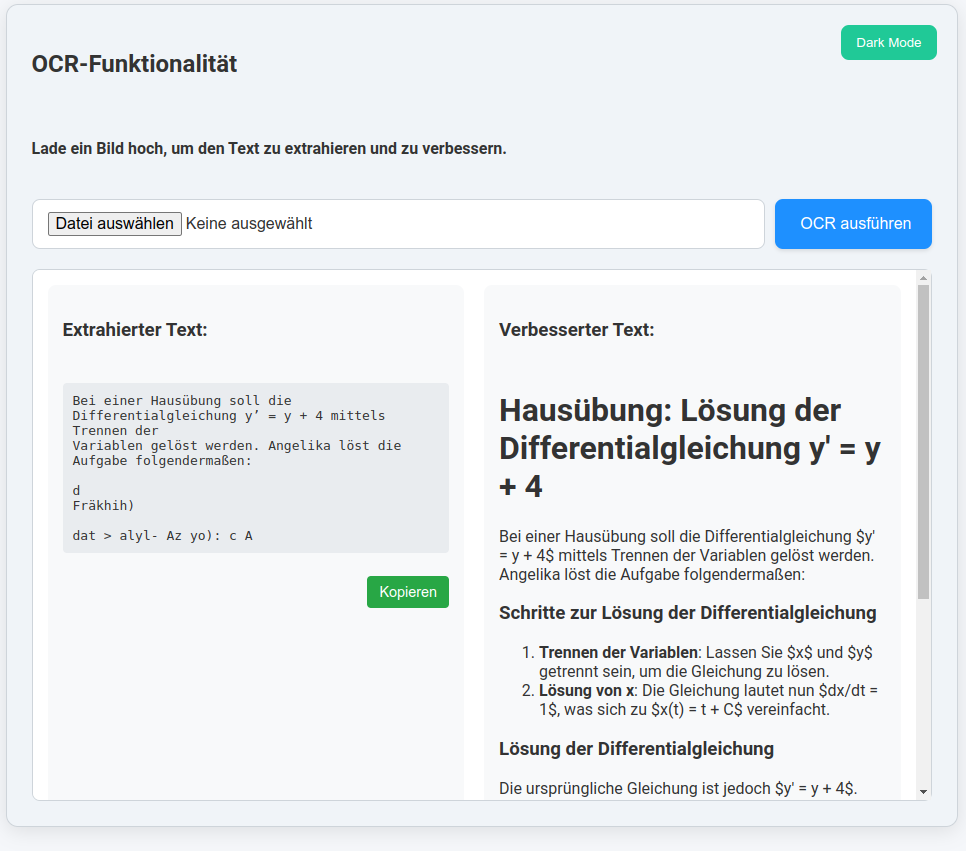
\includegraphics[width=0.6\textwidth]{figures/OCR-functonalatie.png}
  \caption{Image to Text Tool}
  \label{fig:image-to-text-tool}
\end{figure}

The Intelligent Student AI Hub incorporates a dedicated image-to-text tool designed to extract textual information from images. 
This feature first utilizes a text-to-image model to perform optical character recognition (OCR) on uploaded images. Once the raw text is extracted, 
a large language model (LLM) optimizes the content to enhance readability and clarity. The refined text is then presented in a clean, easily accessible format, 
and users have the option to copy the text to their clipboard for further use.

Figure~\ref{fig:image-to-text-tool} \footnote{The image-to-text tool is in German because the platform is designed for students at HTL in Austria.}
illustrates the user interface of the image-to-text tool, highlighting both the image upload mechanism and the display of the extracted text.

The following abbreviated code listing provides a high-level overview of the Vue.js component responsible for handling image uploads, invoking the OCR process via a Flask API, and displaying the processed text:

\begin{lstlisting}[language=html, caption={Abbreviated Vue.js Component for Image-to-Text Conversion}, frame=single]
<template>
  <div class="ocr-component">
    <h2>OCR Functionality</h2>
    <!-- Prompt Input & Image Upload -->
    <input v-model="prompt" placeholder="Enter a prompt..." @keydown.enter="sendRequest" />
    <input type="file" @change="handleImageUpload" accept="image/*" />
    <button @click="sendRequest" :disabled="!selectedImage || loading">
      Submit
    </button>
    <!-- Status and Result Display -->
    <div v-if="loading">Processing image...</div>
    <div v-if="error">{{ error }}</div>
    <div v-if="rawText">
      <h3>Extracted Text:</h3>
      <pre>{{ rawText }}</pre>
      <button @click="copyText(rawText)">Copy</button>
    </div>
  </div>
</template>

<script>
export default {
  data() {
    return {
      prompt: "",
      selectedImage: null,
      rawText: "",
      loading: false,
      error: ""
    };
  },
  methods: {
    handleImageUpload(event) {
      const file = event.target.files[0];
      if (file) this.selectedImage = file;
    },
    async sendRequest() {
      if (!this.prompt || !this.selectedImage) {
        this.error = "Both prompt and image are required.";
        return;
      }
      this.loading = true;
      // Create FormData and send request to the Flask API
      // Response processing updates rawText with extracted and optimized text
      this.loading = false;
    },
    copyText(text) {
      navigator.clipboard.writeText(text);
    }
  }
};
</script>
\end{lstlisting}

This Vue.js component encapsulates the core functionality of the image-to-text tool, enabling users to upload images, extract text content, 
and copy the processed text for further use. By combining OCR capabilities with large language models, 
the platform delivers a powerful and user-friendly tool for extracting textual information from images.

For detailed backend implementation of this tool, please refer to Chapter \ref{cha:hosted_flask_service}, Section \ref{sec:endpoints}.


\section{Saved Chats}

To enhance user experience, the Intelligent Student AI Hub includes a feature that enables users to save their chat interactions with the AI chatbot. This functionality allows users to revisit previous conversations, review the information provided by the AI, and continue their learning journey from where they left off. To achieve this, chat data is stored in Firebase’s Firestore database, ensuring scalable and secure management of user interactions.

\subsection{Implementation of the Saved Chats Feature}

The following abbreviated code snippet provides an overview of how chat messages are stored and retrieved from Firestore. This example demonstrates the core functionality, including loading the list of saved chats, displaying the current chat, and saving updates to Firestore.

\begin{lstlisting}[language=JavaScript, caption={Abbreviated Implementation of the Saved Chats Feature}, frame=single]
<template>
  <div class="chat-container">
    <!-- Chat Window -->
    <div class="chat-window" v-if="currentChat">
      <div v-for="msg in currentChat.messages" :key="msg.id" :class="msg.type">
        <p v-if="msg.type==='user'">{{ msg.text }}</p>
        <div v-else v-html="renderMarkdown(msg.text)"></div>
      </div>
    </div>
    <!-- Sidebar for Saved Chats -->
    <aside class="chat-sidebar">
      <ul>
        <li v-for="chat in chats" :key="chat.id" @click="loadChat(chat.id)">
          {{ chat.name }}
        </li>
      </ul>
      <button @click="startNewChat">+ New Chat</button>
    </aside>
  </div>
</template>

<script>
import firebase from 'firebase/app';
import 'firebase/firestore';

export default {
  data() {
    return {
      chats: [],
      currentChat: null
    };
  },
  methods: {
    async loadChatList() {
      const snapshot = await firebase.firestore().collection('chats').get();
      this.chats = snapshot.docs.map(doc => ({ id: doc.id, ...doc.data() }));
    },
    async loadChat(chatId) {
      const doc = await firebase.firestore().collection('chats')
      .doc(chatId).get();
      this.currentChat = { id: doc.id, ...doc.data() };
    },
    async saveChat() {
      if (this.currentChat) {
        await firebase.firestore().collection('chats')
        .doc(this.currentChat.id)
          .set(this.currentChat);
      }
    },
    startNewChat() {
      // Create a new chat session and persist it to Firestore.
    },
    renderMarkdown(text) {
      // Convert Markdown text to HTML.
    }
  },
  mounted() {
    this.loadChatList();
  }
};
</script>
\end{lstlisting}

This concise implementation outlines how the platform leverages Firestore to manage and persist chat sessions, providing users with a seamless and consistent learning experience.

\section{Structured and Intuitive Navigation}

The platform's navigation is designed to ensure that users can efficiently access desired content and features. To achieve this, the primary components of the platform are placed in the main navigation bar at the top of the page. These key elements include:

\begin{itemize}
    \item Home: Overview of the platform
    \item Account: User Profile
    \item Chat Bots: Selection of available chat bots
    \item OCR: Image-to-Text Conversion
    \item OpenAI Image: Image Genderation with OpenAI
    \item Logout
\end{itemize}

\begin{figure}[H]
    \centering
    
\includegraphics[width=1\textwidth]{figures/Navigation-Bar-top.png}
    \caption{Main Navigation Bar}
    \label{fig:main_navigation_bar}
\end{figure}

To enhance usability when interacting with chat bots, the platform provides a dedicated Chat Bot Section. Within this section, users can select from different chat bots via a navigation bar located on the left side of the page, ensuring an intuitive and structured browsing experience.

\begin{figure}[H]
    \centering
    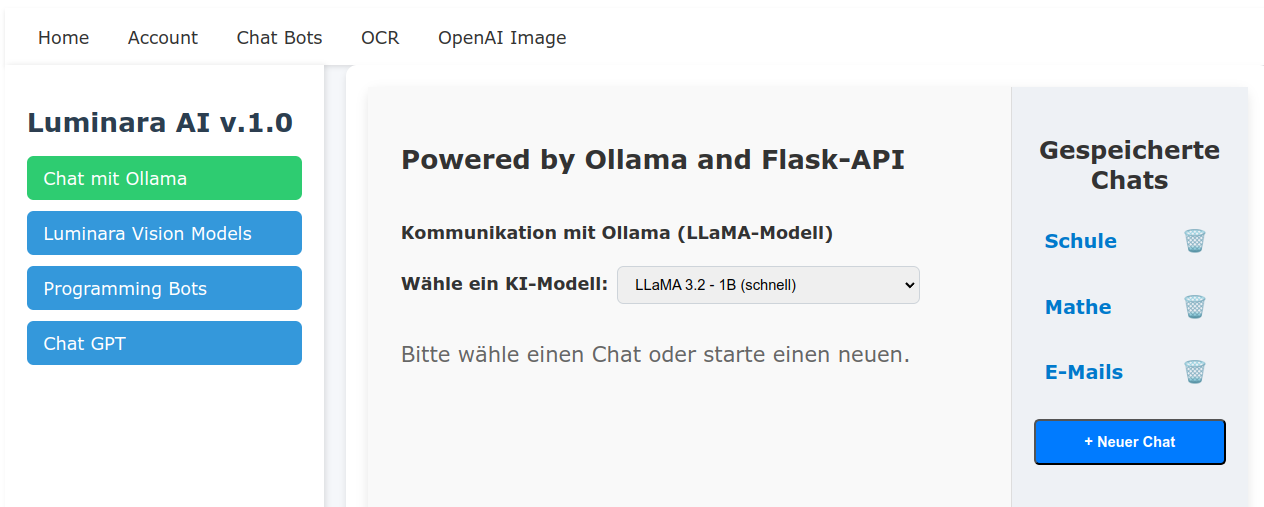
\includegraphics[width=0.9\textwidth]{figures/Chat-Bot-Navigation-Bar.png}
    \caption{Chat Bot Navigation}
    \label{fig:chat_bot_navigation}
\end{figure}

\section{Styling and Theming}

The platform's design follows a clean and modern aesthetic. 
To achieve this, a light and contemporary color scheme has been implemented. The background is predominantly white, 
with blue serving as the primary accent color and green used for highlights. 
For instance, buttons are styled in blue, while the currently selected chat bot is indicated in green. As seen in
Figure~\ref{fig:main_navigation_bar} and Figure~\ref{fig:chat_bot_navigation}.

Most of the styling was implemented using a CSS framework, with initial specifications defined by the development team. These were later refined with the assistance of AI tools, including ChatGPT (versions 3.5, 4, 4o, and o1) as well as GitHub Copilot.

\section{Features Excluded from the Final Version}

Due to the limited development time and the emphasis on core functionalities, several planned features were not incorporated into the final version of the Student AI Hub. These include:

\begin{itemize}
\item \textbf{Multilingual Website:} While the platform currently supports multiple languages for the chatbot, the website itself is only available in German.
\item \textbf{Chat Transcripts:} A feature designed to convert a user's chat history into a downloadable transcript for review and reference.
\item \textbf{Test Preparation:} A module intended to generate practice tests and quizzes based on user preferences and learning progress.
\item \textbf{Learning Analytics:} Tools for tracking and analyzing user learning patterns, progress, and areas for improvement.
\item \textbf{Collaborative Learning:} Features enabling users to collaborate on projects, share knowledge, and engage in group learning activities.
\item \textbf{Enhanced User Profiles:} Additional profile customization options, learning preferences, and progress tracking capabilities.
\item \textbf{Dark Mode:} An alternative color scheme for the platform to reduce eye strain and improve readability in low-light environments.
\end{itemize}

The majority of these planned features were not implemented due to their time-intensive nature. For instance, the development of a multilingual website would have required extensive effort to translate and maintain all website content.

\section{Conclusion}

The Intelligent Student AI Hub represents a significant advancement in educational technology, 
providing students with a comprehensive and interactive platform to explore and learn about Artificial Intelligence. 
By integrating state-of-the-art technologies such as Vue.js, Flask, Firebase, and advanced AI models from OpenAI and Ollama, 
the platform offers a robust and scalable solution for AI education.

The core functionalities—including interactive chatbots, programming assistance, image recognition, 
and image-to-text conversion are designed to enhance the learning experience by making complex AI concepts accessible and engaging. 
The secure and personalized user management system, powered by Firebase, ensures that users can safely interact with the platform while enjoying a tailored educational journey.

While some planned features were not included in the final version due to time constraints, the platform's modular architecture allows for future enhancements and scalability.
Potential future developments include multilingual support, collaborative learning tools, and advanced learning analytics, 
which will further enrich the educational experience.

In summary, the Intelligent Student AI Hub exemplifies the transformative potential of integrating contemporary web technologies
with Artificial Intelligence to cultivate a dynamic and effective learning environment. This platform not only enables students 
to explore the realm of AI but also establishes a foundation for ongoing enhancement and innovation in educational tools. 


